
\documentclass[cropmarks, frame, english]{idamasterthesis}

\usepackage{amsmath}
\usepackage{float}
\author{Paul Nedstrand \& Razmus Lindgren}
\titleenglish{Test Data Post-Processing and Analysis of LA}
\titleswedish{Svensken Titel}
\publicationmonth{THEMONTH}
\publicationyear{2015}
\isbn{ISBN}
\thesisnumber{THESISNUMBER}
\thesisyearnumber{THESISYEARNUMBER}
\dateofpublication{\today}
\supervisor{Ola Leifler}
\examiner{Johannes Schmidt}
\degreesubject{Engineering}
\graphicspath{ {images/} }


\newcommand{\abbrlabel}[1]{\makebox[3cm][l]{\textbf{#1}\ \dotfill}}
\newenvironment{abbreviations}{\begin{list}{}{\renewcommand{\makelabel}{\abbrlabel}}}{\end{list}}


\abstract{
\S\ This master thesis involves developing a lightweight analysis tool that produce statistics in form of graphs from the traffic data in the communication link between a UE, e.g. a cell phone, and a base station which the cell phone is connected to.
The analysis tool will produce graphs with information about the correlation between two signal data in the channel (e.g throughput over interference).
From the statistics produced by the analysis tool, the testing personnel at Ericsson can easily detect potential faulty behaviour from the UE or eNodeB in a more exact way than they were able to do before. This tool will also be able to help Ericsson rewrite test cases from being pretty basic to cover a larger area. The tool will mainly be oriented on analysing link adaptation and HARQ. To show that that it is possible to do an analysis on link adaptation with this tool and to also give an example how to extend testing even further, we made our own analysis on the link adaptations BLER target. This way we could also validate that our tool could handle large amount of data and that you can compare different data with each other.
To be able to show that our tool is usable for Ericsson IODT right now we let IODT test engineers do tests on Link adaptation and HARQ with our tool and evaluate it with their current methods.
}



\begin{document}
\makeintropages

\chapter*{Acknowledgements}
We want to thank our supervisor Sonia Sanghari and Roland Sevegran for giving us the opportunity to make this master thesis available to us and for helping us with material we needed to be able to do this thesis. They have provided us with a lot of help with contacts on Ericsson and with information about LTE.
We also want to thank the whole testing team at Ericsson IODT, for the help we got while doing simulations and also for giving relevant information about the LTE system.

\chapter*{Abbreviations}

\begin{abbreviations}
\item[CQI] Channel Quality Index.
\item[SINR] Signal to Interference plus Noise Ratio
\item[eNodeB] e-UTRA Node-B...
\item[e-UTRA] evolved UMTS Terrestrial Radio Access
\item[e-UTRAN] evolved UMTS Terrestrial Radio Access Network
\item[UE] User Equipment
\item[LTE] Long Term Evolution
\item[MCS] modulation and coding scheme
\item[LA] Link Adaptation,
\item[3GPP] Third Generation Partnership Project
\item[FEC] Forward Error Correction.
\item[OFDMA] Orthogonal Frequency DeMultiplexing Access.
\item[OFDMA Symbol] Orthogonal Frequency DeMultiplexing Access Symbol
\item[DL] Downlink
\item[UL] Uplink
\item[BLER] BLock Error Rate
\item[IODT] InterOperability Design Test
\item[text] text
\item[text] text
\item[text] text




\end{abbreviations}








\chapter{Introduction} %chapter 1
\section{Background}

In a network business, where offering clients help with analyzing UE's performance, having good analyzation tools are important. A UE (user equipment) can be anything that is attached to the network, i.e a cell phone. 

3GPP is a organization that offers requirements for how a network has to perform to be called LTE, but validating this is up to the companies that wishes to create a LTE-network. Therefore, having a good and robust system for testing a UE is a must for companies like Ericsson which offer clients such testing functionality in their labs.
IODT (interoperability design test) is such a section at Ericsson where clients can test and validate whether their UE's lives up to the expectations that LTE demands or not.

3GPP updates its definition of LTE regularly, so testing a system only once if it is fulfilling the requirements of the LTE network standards does not guarantee that it will always be compatible. The same can be said about the tools that IODT uses for testing, they have to be dynamic enough in their functionality to allow different types of tests to be run in the same program so that they don't have to write a new testing-tool whenever there comes out a new type of test-requirement from 3GPP.

Some of the testing has been performed by manually analyzing small chunks of signal-data. Since analyzing an entire file with trace-data could take a lot of time and also creates a risk of faulty analysations, Ericsson requested a new type of tool which would enable the testers to get a good view of how the data in large files behaved without them having to manually read through the entire log file with traffic data. This is also the task that was given to us as our examination thesis.
\newpage

\section{Problem Formulation}
Ericsson IODT does not currently have any tool or functionality to make analysis of data of the air interface data in LTE for testing in a more indepth way. The way the testing department IODT works is that they manually look at log files for potential problem in the link between the cell phone and base station. These files often contain a lot of data and can be quite hard to analyze, it is then difficult to see and detect potential problems or to see the performance of the UE. The other way they study data is to look at it in real time in a command window, which goes with a very high speed, which makes it easy to miss potentially faulty behaviour. There is hence no way to make an in-depth analysis or post analysis of HARQ and link adaptation data in the air interface, so it would be very hard or nearly impossible to detect errors that would occur only a few times. An example of an error could be that the UE stop sending traffic under a short period of time or that the receiver didn't understood a specific message but the transmitter ignored it (byt ut sista exemplet till natt bra). There is also a need to look at and compare different UE's performance to each other or the performance on the same UE with different setups, but there is currently no method to do this in a good way. \newline

The questions this thesis seeks to answer is
\begin{itemize}
\item How can we help  IODT to do post analysis especially of link adaptation and HARQ in an efficient and (good?) way that helps them to detect error and faulty behaviour?

\item Can we provide Ericsson with a better alternative to look at and  compare performance between different UE's (or same UE with different setups) instead of by looking up the values manually in logfiles?
\end{itemize}




\section{Related Work}
tabort?

\section{Thesis Outline}
This thesis is divided into the following Parts
\begin{itemize}
\item Chapter 2: Theoretical background: In this chapter we explain all thoertical background needed to understand this thisis.
\item Chapter 3: Method: In this chapter it is described how we proceeded to solve the problem we were given.
\item Chapter 4: The analysis tool: In this chapter it is described how the tool works, and the motivation behind functionality of it.
\item Chapter 5: The analysis: In this chapter it is describes in detail the analysis we did with the tool.
\item Chapter 6: Future work: In this chapter we write about how the tool can be developed even further.
\item Chapter 7: Conclusion: In this chapter we write about our conclusion of the project.
\end{itemize}






















\chapter{Theoretical Background} %chapter 2
In this chapter the theoretical background is described to fully understand this thesis.


%vi bor skita i detta
\section{LTE and eUTRAN}
LTE stands for long term evolution and is the access network in the evolved package system (EPS) and was introduced in 2008, it is also known as 4G but has yet to fulfill some requirements to call itself that [source] so instead it is referred as 3.9G. The reqirement of LTE is high peak data rate, high spectral efficiency and flexible frequency and bandwidth [4].
\\
eUTRAN stands for Evolved Universal Mobile Telecommunications System Terrestrial Radio Access Network, or just Evolved UMTS Terrestrial Radio Access Network. The eutran consist of a network of eNodeB's that are connected to each other. It is the archtecture defined as the eutran...

\begin{figure}[H]
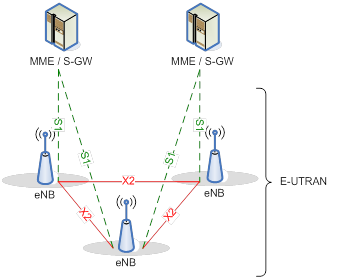
\includegraphics[width=\textwidth]{eUtran_[36300-c20]}
\centering
\caption{Picture of eUTRAN [7]}
\end{figure}






\section{The physical layer of the LTE System}
The layer we have been working in is called layer 1, also known as the physical layer. It is the description of how the signals are sent through the air, how they are scheduled and how they are modulated (typ). All the parameters that you are able to look at in the tool is in this layer.


\section{Link Adaptation}
Link adaptation is a way to enhance the performance in wireless systems were the channel condition might vary in time [6]. Dependent on the channel condition the modulation scheme and code rate is changed to get this highest performance in throughput as possible. The better channel condition the higher modulation scheme and higher code rate is used and the worse channel condition the lower modulation scheme and higher code rate [source]?. The modulation scheme used in the LTE systems are QPSK, 16QAM and 64QAM. The codes used is QPP (quadrature polynomial permutation) turbo code [source].

\subsection{How it works}
When data is sent from a base station to a UE (DL) the UE will report a CQI (channel quality indicator) value to the eNodeB indicating how good the channel is. CQI can take values from 0 to 15 (4 bits) where each number correspond to a channel condition, 0 represent a very bad channel condition and 15 a very good one. From this value the eNB decides a MCS (modulation and coding scheme). For downlink, MCS can take values between 0-28 and uplink 0-24 [source]. Each one of these values represent a modulation scheme and code rate, were MCS = 0 is when you have the worst channel condition, which has the lowest code rate and lowest modulation order (QPSK) and MCS = 28 in downlink and 24 in uplink has the highest code rate and the highest modulation order (64-QAM) which is on the best channel condition.

LTE is using a so called fast link adaptation. It means it takes both the cqi and BLER into consideration when it is deciding the MCS [6]. An MCS is assigned as a function of CQI and the BLER (block error rate) [source]. First the eNodeB sets an MCS from the CQI value. If the data has the BLER that is assigned in the eNodeB then it will keep the MCS, if the BLER is lower or higher the MCS is adjusted so that this target is achieved. 

In the uplink the same principles are used but instead of looking at a CQI value the mcs is determined directly from the SINR, a high SINR correspond to a good channel condition and vice versa, this means that a high SINR will lead to a high MCS and vice versa.

\subsection{Modulation}
A modulation scheme is a way to map digital bits to analog signals in wireless systems. The analog signals are electromagnetic waves [soruce] and is a way to represent the bits in the air.
There are different modulation schemes and the ones that are used in LTE are 4QAM (QPSK), 16QAM and 64QAM [source]. The signals are modulated in the following way

(bild pa 4QAM 16QAM and 64QAM over I-phase and Q-phase).
The I-phase is basically a Sinus wave and Q-phase is a Cosine wave. What the points on the two axises represent is the the power of the signal [source]. So in the QPSK case, what the different signals will be is:\\
A*sinus(f*t)\\
A*cos(f*t)\\
-A*sinus(f*t) \\
-A*cos(f*t)\\

In this case it fits 2 bits in each signal. Therefore, the different possible signals are 00, 01, 10 and 11. In 16QAM and 64QAM each signal point is represented by 4 and 6 bits respectively.

The signals in LTE are modulated and demodulated with a so called IQ-modulator and IQ-Demodulator. It means how they are transformed from digital to analog, and analog to digital signals.
TODO(write stuff about IQ-Modulator/demodulator)

\subsection{Coding and Code Rate and FEC}
Coding is a way to create redundancy in the data that are sent. The data will consist of real data bits and coded bits. This way you are able to correct bits that are incorrect in the receiver. The more coded bits you have in your message the more errors you can detect and correct, but the slower data rate you will have. The code rate states how many bits that are coded in a message. the Code rate is between 0 and 1 and is simply $\dfrac{\# real bits}{ \# real bits + \# coded bits}$ .
\\ \\
example: if we have a code rate of 0.73 we have 73\% real bits in the message and 27\% coded bits.

The simplest coding scheme is repetition codes. If you want to send the bits 1010. you can instead send 111100011110000. You repeat the bit a fixed number of times. In this example 4 times. If the data is wrongly receiver say that you received 1011000011110010. Then the receiver can see that the 2nd and 15th bit is wrong and can correct these. Therefore you don't have to do a retransmission and you save time. These type of  is called FEC (forward error correction).

\subsection{MCS}
MCS is a key parameter in link adaptation. MCS stands for modulation and coding scheme and it describes how that data is modulated and coded as an analog wave. Every signal has an MCS and this MCS has a specific modulation scheme and coding scheme. In LTE there are several selections of MCS's. There is (currently) 29 different MCS's in the downlink and 25 in the uplink [source]. in LTE each MCS is used in different channel condition. In the best signal conditions the data is sent with MCS 28 in DL and 24 in UL, and in the worst they both have 0. A list of how the data is modulated and coded is below.
\\
Picture on MCS table for uplink and downlink

\subsection{BLER and BLER target}
BLER stands for Block Error Rate and is in this thesis referred as the percentage of the wrongly received blocks in the receiver (UE or eNodeB) [source]. It is defined as $\dfrac{\# wrong received bits}{ \# wrong received bits + \# right received bits}$ [source]. \\

In the eNodeB there is a so called BLER-target, it determines how many bits that on average should be wrongly received. One can argue that it should be best to have a bler target on 0\% or as low as possible but it would be quite expensive. You would have to have a very low MCS to this target, hence the throughput would decrease, the throughput is something that you want to optimize as much as possible. So there is a tradeoff between MCS and BLER if you want to have the highest throughput. The higher BLER-target that is set in eNodeB the higher MCS you will have but the more retransmissions and vice versa.

There are two several bler targets





\section{HARQ Algorithm}
HARQ stands for hybrid automatic repeat request and is an algorithm to handle rightly and wrongly received data. HARQ is a combination of FEC (forward error correction) and ARQ correction control [source]. When data is sent from transmitter to receiver, the data might either be correct, incorrect and correctable or incorrect and incorrectable.

If the data that is sent is correct in the receiver, it will send an ACK bit which then the transmitter receives. ACK stands for acknowledge and means that the data that was sent was understood, and the transmitter can sent new data.

If data is incorrect but correctable the wrongly received bits will be corrected an ack bits will be sent. The number of of bits that can be corrected is dependent on how many code bits you have [source]. The transmitter can send new data

If the data is incorrect and uncorrectable the receiver will send an NACK (Not ACKnowledged) bit and the data will be retransmitted.
(picture on harq ack, harq corrected bit ack och en nack)

Since there will be a delay between when data is transmitted and an ACK/NACK will be received, there are different HARQ process in LTE that are running in parallel. The number of HARQ processes in the LTE standard is set to 8 [source (air interface boken)]. This way the data won't have to halt the data before a new transmission or retransmission but can send new data immediately and resend the wrongly received bits at a later stage.
\\
\\
(picture on the parallel harq process)
\\


\section{Forward error correction}
Forward error correction or FEC is a method to correct messages at the receiver side. Data that is transmitted can either be right, wrong and correctable och wrong and uncorrectable. When the data is wrong and uncorrectable the data must be retransmitted. When data is wrong and correctable FEC is used. This is the reason why you have coded bits in your message. If you know how they

\section{SINR}
SINR stands for Signal to inteference plus noise ratio. It is defined as the powerSignal/(powerInterference + powerNoise). This is a relevant parameter to measure the quality if the channel

\section{CQI}
CQI stand for channel quality indicator and is an indicator of how good the channel is. It is similar to SINR but can only hold 15 different values. Where 15 indicates a very good channel quality and 0 a very bad one [source].


\section{OFDMA}
OFDM stands for orthogonal frequency demultiplexing and is a way to send wireless data in parallel. The principle is that the data that are sending must be orthonormall to each other. To do this the data must be mapped onto subcarriers. These subcarriers must have a frequency of a multiple of f, where f i the sampling period of the receiver. Orthogonormal in this sence means that a integral from 0 to 1/f A x B = 0, if A != B and integral from 0 to 1/f A x A = 1.
if the bits are mapped to these subcarrier, one can send data in parallel...

In LTE this sampling frequency = 15000 Hz. This means that all bits or symbols are mapped to a multiple of of this frequency. ie 15k, 30k, 45k ... 

\section{TBS}
TBS stands for transport block size and tells how many bits that are sent in one scheduled time interval  (TTI) = 1ms. From this value one can easily calculate the throughput of the data that are sending. TBS defined as ...
















\chapter{Method} %chapter 3

\section{Our suggested solution}

Our task from Ericsson was to develop a lightweight analysis tool that produce statistics from data traffic between UE and eNodeB. The tool should be able to handle several input parameters and from these parameters produce data in form of graphs. These parameter could for example be throughput, time, error rate etc. \\
From these produced graphs post analysis of link adaptation and HARQ should be possible.
If we had time we would construct functionality to store graph data, so that one could be able to make comparisons with other UE's performance or the performance of one UE with different settings. \\

\setlength{\parindent}{0cm} To be able to construct this kind of tool of we first needed to know:\\
What kind of data shall we handle and produce graphs from? \\
What quantities of data shall the program be able to handle? \\
What type of statistics are necessary? (max, min, average, dependencies, between parameters etc)

To be able to answer the above questions we needed to:
\begin{itemize}
\item Study the LTE air interface.
\item Learn how data traffic is stored and handled.
\item Learn how data traffic is collected.
\item Study which kind of data parameters will be useful.
\item Evaluate a suitable tool for the processing of data, e.g. MATLAB or something similar.
\item Interview personnel at Ericsson.
\end{itemize}


Ericsson did not have a clear picture of what kind of tool they needed to perform analysis of LA and HARQ. Nor did they have any specification on what type of data that was important to study or any hard criteria on what we should do in our program. Since they didn't have any form of plan for how to perform our work or any criteria on the data we should produce it fell to us to study what the functionality and analysis should be.


\section{How we collected information}
Since Ericsson didn't have a clear picture and few specifications of how the tool was going to be used, our initial approach on how to figure out what we needed to do was to have a focus group with lots of personnel from Ericsson that is directly or indirectly involved with our examination work. That means personnel that came up with this idea, and personnel (employees) that probably will use this tool in the future (mainly test engineers at IODT). \\

We were going to hold a focus group were several of these employees were invited, but few came we couldn't gather enough information like we wanted. Because of the difficulty in organizing official meetings, since some of the employees works in in different cities and have a lot of other things to do, we instead talked to personnel one at a time continuously as our work progressed to ensure that what we currently were implementing reflected what they needed.

\section{Literature}

To understand the data that we were suppose to handle and plot we had to understand the parameters in the traces and what they mean. We did this by reading books given by Ericsson about 3gpp and LTE. \\

Academic Press 3G Evolution HSPA and LTE for Mobile Broadband 2nd Edition Oct 2008 eBook-DDU, describes LTE amongst other topics in detail. \\

Ericsson Academy LTE L11 Air interface. Explains how the signals are sent through the air,  explains modulation, the HARQ procedure, uplink, downlink, OFDM, which is relevant when working in this area. This way we more easily understand how the tracedata would look like.

We also talked to IODT test engineers at Ericsson who were knowledgeable in LTE and could explain different parameters in the data traffic.

To better understand on how to perform analysis on link adaptiation an HARQ, we read the following scientific articles on analysis of LA and HARQ:

Overview of ARQ and HARQ in Beyond 3G Systems. Antonio Maria Cipriano, Paul Gagneur Guillaume Vivier, Serdar Sezginer, 2010.

Performance Analysis of Link Adaptation in LTE Systems, Tao Tao, Andreas Czylwik, 2011.

Performance Comparison of Type I, II and III Hybrid ARQ Schemes over AWGN Channels, M. Wissem El Bahri, Hatem Boujemgaa, Mohamed Siala, 2004.

To be able to know how to do focus groups we used the article 
Zane K. Quible, A Focus on Focus Groups, Stillwater, Oklahoma State University, 1998.


\section{testing and validating our tool}

To validate that we had implemented our tool in a correct way we set up a set of goals:
\begin{itemize}
\item Can our tool provide functionality that is useful to the testers?
\item Can a tester get more exact result with our tool than without it?
\item Can an analysis on LA or HARQ be performed with our tool?
\end{itemize}



\subsection{Test analysis on  BLER target}
To test and see if our tool worked as we intended we did a test analysis of the BLER target assigned in the enodeB. We wanted to compare different traces to data with the same channel condition and on the same mobile phone but with different BLER targets. If you change the BLER target some of the parameters in the data traffic would change in an expected way, how these parameters are correlated to each other are explained later, therefore we could find more potential errors or potentially incorrectly drawn graphs in the tool than you would if the setting would be the same. We would also clearly see if there were any parameters missing to be able to this analysis compared to if we analysed something that didn't relate to link adaptation. \\

At first we compared the results from each BLER target test in the same graph to see whether our the curves looked as they should, this would be a good indicator whether the curves were drawn correctly or not. A test were made were we looked at points in the graph and compared these to what they should be (by calculating it manually in excel). 
We also  wanted to see if the tool could handle and plot several trace files (.csv) at the same time in the same graph.


\section{Validating the tool}

To validate that our tool is useful right now and not only a potential future work of analysis we felt that we had to do a test with their current methods and compare it with our tool. There is right now quite few test that needs a graphical representation, the most relevant we found is a test on link adaptation and HARQ.

\subsection{Survey}
To be able to ensure that the tool can come into work soon we let testing engineers at Ericsson IODT use our tool. What we wanted to do was to measure how good our tool was. The way the testers work is that they manually look at the log file, so our comparison is with that. We created a survey where we asked questions of what the testers felt of the tool. The survey is available in the appendix.


\section{measurements result}
text













\chapter{The Analysis Tool} %chapter 4
Our analysis tool was developed for IODT at Ericsson. The purpose of the tool was to analyze data in layer 1/physical layers, especially LA and HARQ. It has been developed so that IODT in an easier way can do a post analysis of the data traffic between the UE and eNodeB. \\


The tool is mainly developed to perform analysis of data over SINR and CQI, i.e. the channel condition. But it is also able to use all parameters (that are sent between the UE and eNodeB) as an axis in graphs so that the tester can validate any data he/she wants. The tool also allows the user to compare multiple datasets so that different UEs easily can be compared to each other. \\

The tool is built on top of an already existing program called Logtool, and is written in the program language Java. 

\section{Motivation for choosing Logtool}
In the beginning of the project we had to take a decision on how we would create our analysis tool.
What we needed to do was produce a program that would:
\begin{itemize}
\item Read trace data in form of logfiles%vilka resources?
\item Plot graphs with data from the analysis
\end{itemize}

We came up with these questions that we felt was necessary to answer in order to produce a useful tool :
\begin{itemize}
\item Can IODT testers study and analyze the layer 1 data (especially link adaptation and HARQ) with our tool?
\item Is it easier to get a better overview of large quantities of trace data than it was before?
\item Is it easier to get a better overview of small quantities of trace data than it was before?
\end{itemize}

Since we didn't have any requirement on how we should implement our tool we decided that ourselves. We felt that the best way was to build it upon an already existing project or in an environment that already had the functionality to do everything we needed. \newline
We started to analyse available (already existing) tools by asking personnel at Ericsson if they had any preferences or any tools that they knew that they already had licences for or tools that was already used in the lab testers environment. Unfortunately they didn't have any recommendations, so we started to search the web for good tools that would be able to produce graphs and analyze big sets of data. Our initial idea was Matlab since both of us have experience with Matlab and it contains extensive libraries for calculating signal data and for plotting graphs. We investigated other Matlab-like tools, but mostly all other programs seemed to do pretty much what Matlab did or less, and since we already had experience with Matlab we concluded that Matlab was our best choice. \\
We were still pretty open minded about using other softwares at this point, but started out with just writing code for displaying graphs. After about a week we found out from our supervisor that Ericsson did indeed already have a Ericsson-developed program called Logtool that the lab testers used for handling tracedata. It was written in java and the program was built upon the eclipse framework, all of which Razmus already had experience with since earlier. The team in charge of the project was in Link\"{o}ping, and using Logtool would enable us to get tracedata in a good format without us having to write code to extract data from the raw log file, plus our program wouldn't need any form of extra integration for Ericsson. Another good thing with developing the tool in logtool is that all ericsson employees has access to it.
We therefore decided to develop our program as a plugin to Logtool.
%beratta om bb-filter redan här!

\section{Logtool Plugin}
Logtool is a program that contains different analyzers that does individual analysis on raw trace data. Each analyser that the project uses is added as a plugin-project and not directly integrated into the project. We needed the raw trace data in a BB-filtered (BaseBand-filtered) format, and it existed a plugin which already did that. We could have written our project as a new plugin but both we and Ericsson were agreed on that it would be unnecessary to implement a new plugin which would need to BB-filter the data when that functionality already existed and also if we did that the data that bb-filter produce wouldn't be available.

\section{Description of the Tool}
Ericsson first requested us to do an analysis tool that would plot graphs in a basic interface. We included extra functionality and created a total of 3 different kinds of views (a separate window in eclipse) with unique functionality. The first view just contains a set of graphs that the user can save to file. The second view uses saved graph data to plot it in the same layout of graphs as the first view does, but it can load multiple datasets at the same time which allows for smooth dataset comparisons between different trace files. The third view is a more dynamic view that allows the user to load .csv-files and create any form of graph with the parameters that exists in the file. It also has the capability to handle several files at the same time so that the testers can compare multiple UEs at the same time and to easier detect errors.


\subsection{BasicView}

\begin{figure}[H]
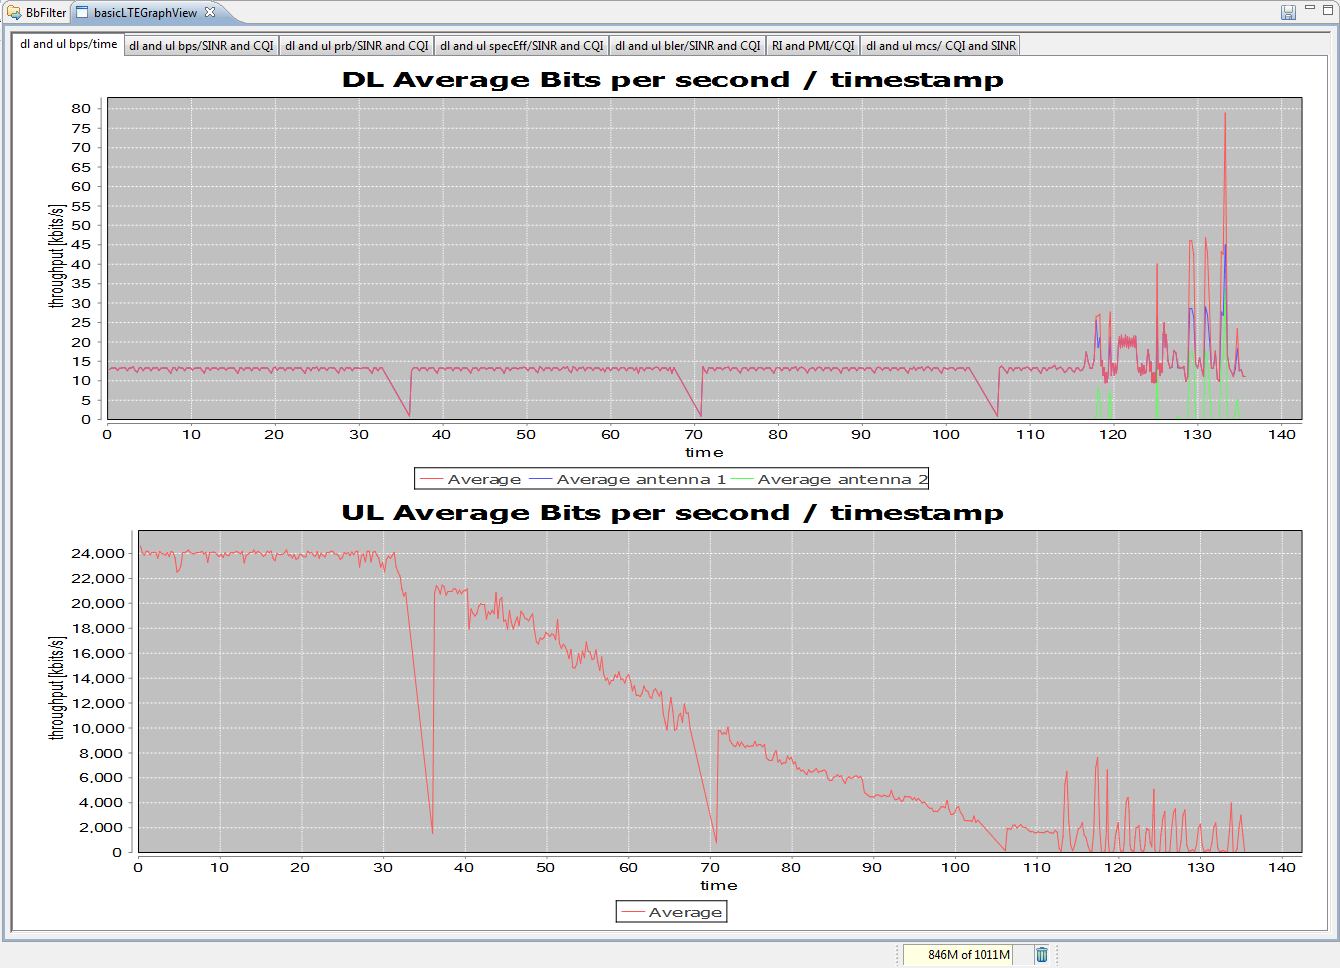
\includegraphics[width=\textwidth]{BasicView}
\centering
\caption{Picture of the basic graphs view [7]}
\end{figure}

The first view contains a fixed set of graphs that shows certain data that is useful for testers to quickly get a good picture of how the data looks like. The main type of data shown in these graphs are different parameters that has a dependency to SINR and CQI plotted over SINR and CQI (CQI is for downlink and SINR is for uplink). These values we got as suggestions from Rickard Wahlgren and Jonas Wiorek, they are two Ericsson employees at Kista that has a good insight in layer 1 and also came up with this thesis idea. The reason for why we look at SINR in uplink and CQI downlink is because the UE doesn't calculate SINR, it calculates CQI which can be translated as a SINR but it only contains 15 values. \\

The graphs you can look at is Throughput/SINR, Throughput/CQI, PRB/CQI PRB/SINR BLER/CQI, BLER/SINR, SINR/(UL MCS) CQI/(DL MCS) ... These graph are presented in a two dimensional graph as showed in picture X. Where the data is on the Y-axis (vertical axis) and SINR / CQI is on the X-axis (horizontal axis). \\

The graphs are all calculated as the average value over the corresponding SINR or CQI. We first thought that it might be good to show max and min curves as well as the average. But we skipped this idea since we realized that the graphs would contain too much information if you load in several sets of data and it would be hard to separate them. This was also not a requirement from Ericsson. \\ 

The user can save the graphs  to file (as a .graphdata file) which just contains the actual graphdata and not the whole data that were used to produce the graphs. This makes the file very small compared to how the file would have been if all raw data would have been saved to file which saves a lot of storage space.


\subsection{Multiple Graph View}
	
\begin{figure}[H]
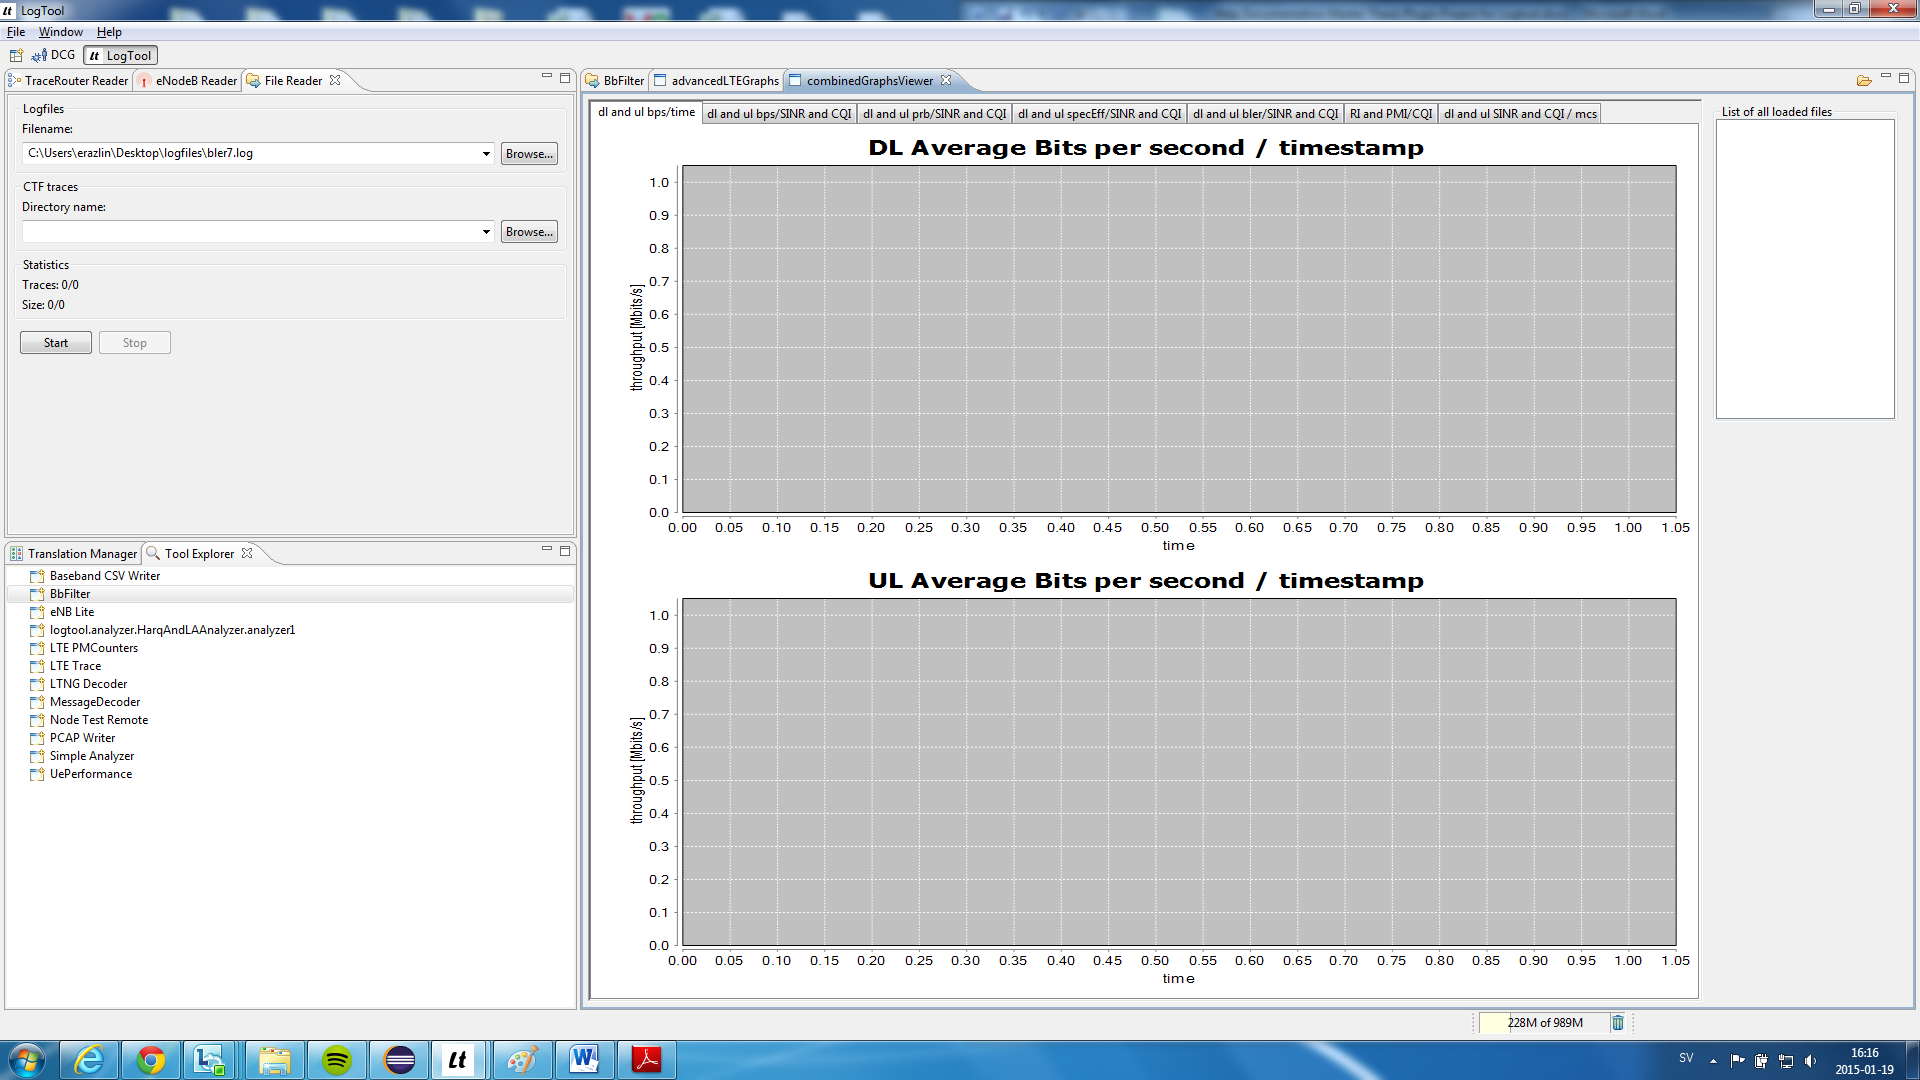
\includegraphics[width=\textwidth]{CombinedGraphsView}
\centering
\caption{Picture of the combined graphs view}
\end{figure}

The second view contains the functionality to load graphs saved in BasicView, if you have two sets of data you should be able to compare them. There is a save button in the BasicView, after you have saved your graphs you can run several other bb-filtrations and save those graphs too. The user can then load all the saved graph datasets that you wish to compare. Each loaded dataset can be toggled on/off through a list in the right corner of the view. 

This view was created only to offer some supporting visualization to the BasicView rather than being whole new view with lots of unique functionality.


\subsection{AdvancedView}
	
\begin{figure}[H]
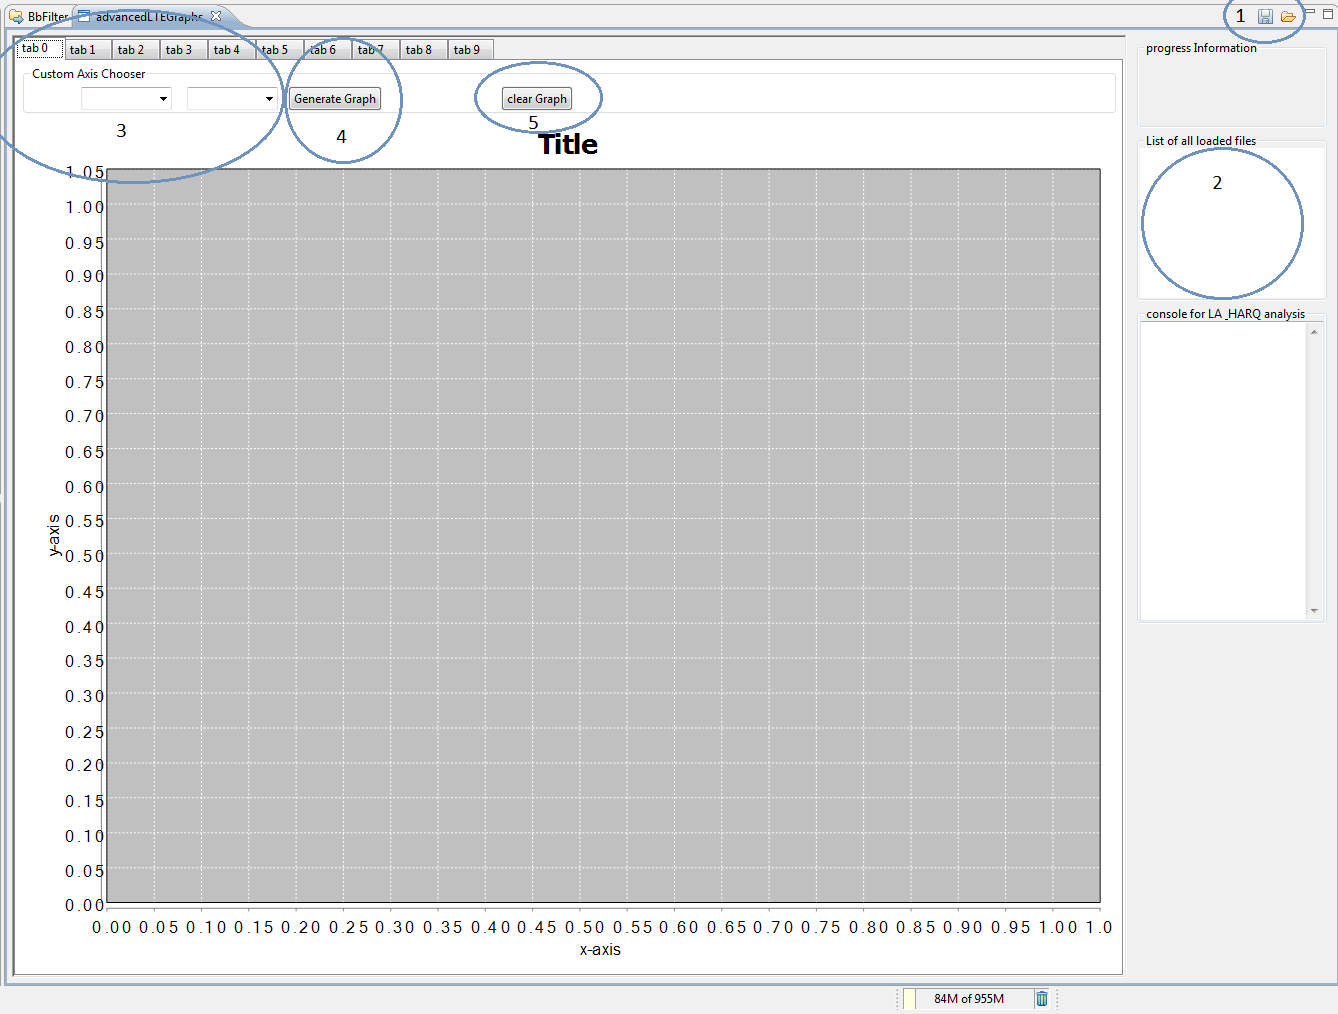
\includegraphics[width=\textwidth]{AdvancedView}
\centering
\caption{Picture of the Advanced graphs view}
\end{figure}

The third view is what we call the AdvancedView. In this view you are able to look at data in any form of graph where you choose what you want to look at in the X and Y-axis, and then plot your graph over those values. We got this idea from a tester in the lab. We implemented this because we thought this tool could be used in other areas as well rather than just in link adaptation / HARQ. To only have graphs over SINR and CQI might be too narrow. \\



\subsubsection{1 - Load / Save}
If the user has bbfiltered any data in the BBFilter view and then opened AdvancedView, then that data can be saved to a .csv file by clicking on the save button. \\
The user can also load .csv files by clicking the load button. It requires the files to have the same parameters as the first loaded file otherwise the file will not be loaded.

\subsubsection{2 - Files In Use}
When a file has been loaded it is then added as an object in the loaded files list. That object can be checked/unchecked to decide if data should be collected from that file when generating a new graph.
	
\begin{figure}[H]
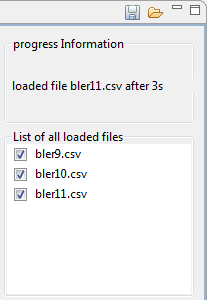
\includegraphics[scale=0.7]{AdvancedView_LoadedFiles}
\centering
\caption{List of loaded files}
\end{figure}

\subsubsection{3 - Axis Parameters}
Each DDL(drop down list) contains the parameters that are stored in the first loaded .csv file.The user selects a parameter of choice for both the x- and y-axis.

\begin{figure}[H]
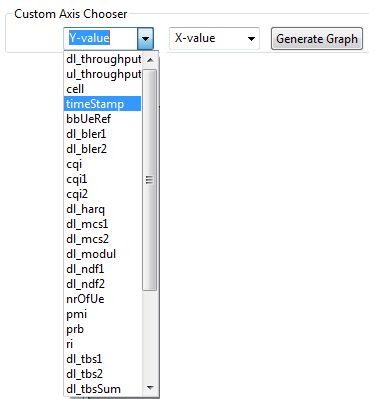
\includegraphics[scale=0.7]{Axis_Parameters}
\centering
\caption{Available axis parameters in the custom axis DLL's}
\end{figure}

\subsubsection{4 - Graph Generator}
When the user has selected 2 axis-parameters in the DDL, then he/she presses the "Generate Graph"-button to start the process of calculating data for the graph and also for plotting the data in the graph.

\begin{figure}[H]

\includegraphics[scale=0.7]{Generate_Graph}
\centering
\caption{The Generate Graph button}
\end{figure}

\subsubsection{5 - Graph Remover}
When a user has generated a graph then the data stays in that graph until the user presses the "Clear Graph"-button. This is because a user might want to have 2 different kinds of graph data in the same graph, so the user has to manually clear the graph when he/she needs to.

\begin{figure}[H]

\includegraphics[scale=0.7]{Clear_Graph}
\centering
\caption{The Clear Graph Button}
\end{figure}

\subsubsection{Time Axis Compresser}
We also implemented a function that compresses the time-axis into smaller segments, we did this because the graphs that are plotted over time can contain around 140 000 x-axis points which makes the graph a bit messy. What the function does is that it takes a compression-value that the user sets in a textfield (default is 100) and then compresses that amount of old values into a single new point. That is, if you have 140 000 values in the graph and chooses compress-value 100, that would make the new graph contain 1400 points instead of 140 000 which is a lot easier to read. \\

The compresser-value is only visible when "timeStamp" is choosen in one of the custom axis DDL's.\\

The compresser-value can be set by changing the value in the textbox in the image below.
\begin{figure}[H]
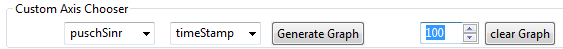
\includegraphics[scale=0.7]{AdvancedView_TimeConstant_Marked}
\centering
\caption{Compresser-constant value box}
\end{figure}

On the next page is an example how the compresser-constant can be used to make data more readable.
\newpage

Here is a graph where SINR is plotted over time
\begin{figure}[H]
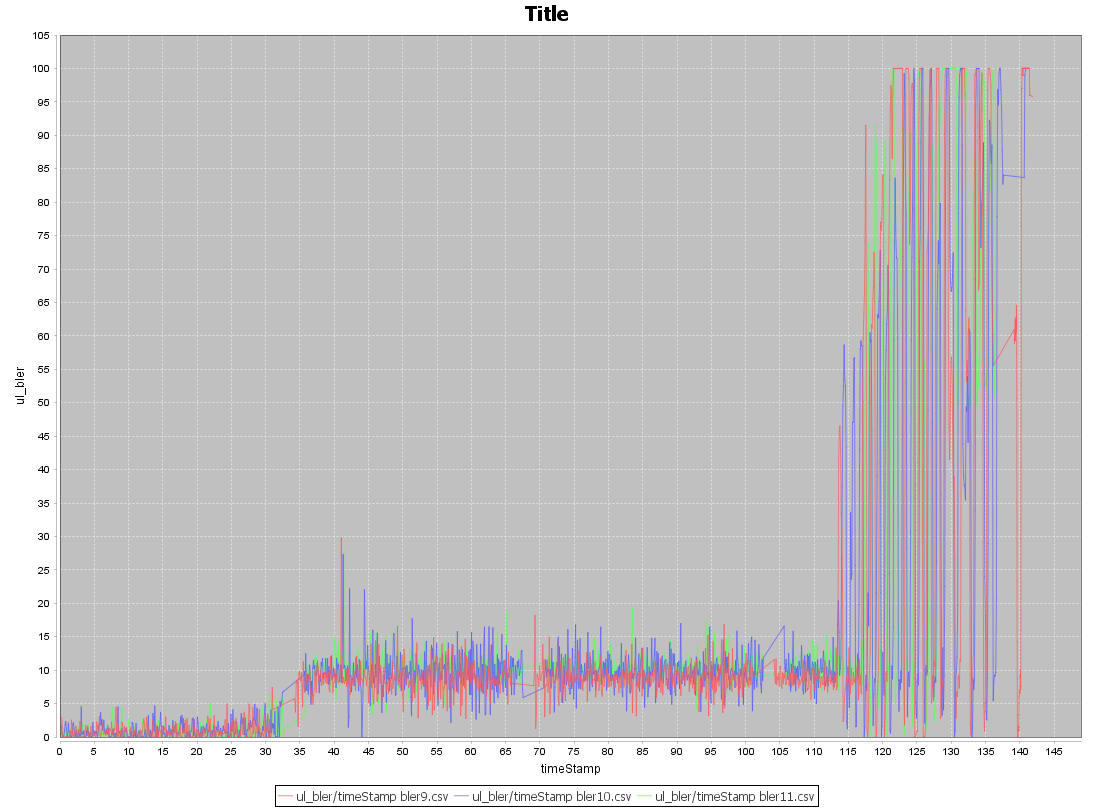
\includegraphics[scale=0.25]{AdvancedView_bler_over_100}
\centering
\caption{Generated graph with compresser-constant set to default(100)}
\end{figure}

Here is the same graph but with compresser-value 2000
\begin{figure}[H]
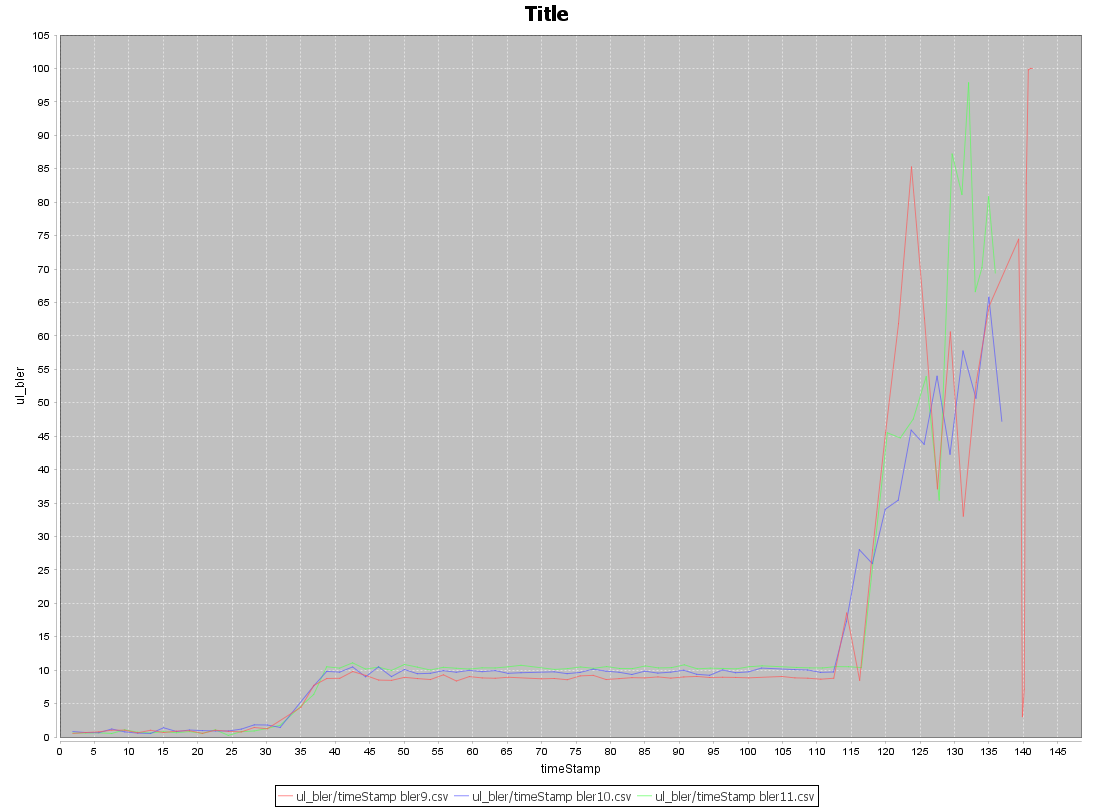
\includegraphics[scale=0.25]{AdvancedView_bler_over_2000}
\centering
\caption{Generated graph with compresser-constant set to 2000}
\end{figure}

It is quite easy to see that the difference in readability is quite large between the two graphs.


























\chapter{The test analysis of BLER target} %chapter 5
In this chapter the analysis of the BLER target is formulated, the reason behind the analysis, how we did it and a summary of it.

\section{Motivation}
The reason why we did this analysis was to validate that our tool works as we have intended, that we are able to read several files at once, that it can handle the size of the data that we wanted and the it shows the right data. We also wanted to show that a relevant analysis on link adaptation is possible, meaning that we put the tool in a relevant context.

What we wanted to verify was:

Can the tool can handle data from different from different traces.\\
Can the tool handle larger files without memory problems. \\
Does the graphs produce the right data. \\
Are you able to do a relevant analysis, meaning that you are able to study something and draw conclusions from it \\





\section{explanation the BLER analysis}
The analysis we have done is on the performance of different BLER targets. We did this analysis because the BLER target is a key relevant parameter in link adaptation [source], so we believed it would a relevant context. In the eNodeB there is a BLER target set for the data that is sent in downlink and uplink. This means that the data should keep this BLER regardless if the channel conditions are good or bad. You change your modulation and coding scheme (MCS) until the BLER target is achieved. How the MCS affects BLER and throughput are explained earlier in the thesis. So there is a tradeoff between different BLER-targets if you want achieve the highest throughput. The higher BLER target you have the higher number of bits can be sent, but you will have more retransmissions. The lower BLER target you have the lower block sizes but lower retransmission.

In the eNodeB's at Ericsson's test lab the BLER target is at 10\% as default. Is this the optimal target rate if you want to achieve the highest throughput? To analyze this we extracted several Basebands traces with the same channel conditions. To do this we used a script that an employee in Ericsson had done before, which switch the SINR in the channel with the same time interval. So the first traces we collected was on BLER 10\% (which is default) were we switched the SINR from 20 dB to -15 dB??, were each SINR is held in four
seconds. The reason why this script is used is to both to achieve as similar environment and to be able to better compare the data over time.

The question we want to answer in the analysis is:
Is the BLER target at 10\% the optimal one, meaning does it have the highest throughput.
Are there any difference between the throughput over different SINR's and the traces.

\section{The simulated channel and channel model}
The channel model we used for the simulation was called $2x2_1x2$ static. It means that the eNodeB has 2 transmitting antenna and the UE in this cell phone has 2 receiving antenna and the cell phone has 1 transmitting antenna and eNodeB has 2 transmitting antenna. Static means that the cell phones is not moving. The Channel is of the type AWGN (additive white gaussian noise). This is the more common channel type and it is used to mimic natural behaviour.
'Additive' because it is added to any noise that might be intrinsic to the information system.
'White' refers to idea that it has uniform power across the frequency band for the information system.
'Gaussian' because it has a normal distribution in the time domain with an average time domain value of zero.
This channel model was used basically because it is a common situation how the cell phone are sending data to a eNodeB. The reason why we choose uplink was because we get the SINR is calculated. Only a CQI calculated in downlink, so we get more values to plot over in in the uplink over SINR werwer.


\section{How we collected data}
We collected the data by connecting the cell phone to an eNodeB, start the data traffic and turn
on script that change the channel condition, recorded the data and saved it to a file. We did this procedure for different BLER target settings in the eNodeB. The BLER target we used was 1\%, 5\%, 7\%, 9\%, 11\%, 13\%, 20\%, 35\%. By comparing a lot of data we could also varify that we can handle a lot of traces. The traces are stored as raw log files. \\

picture of the content of a raw file.

\section{How we read the data}
We read the data with the analyzer bbfilter in logtool which translate the raw log file to csv format\\

picture on bb-filter data.

From this data you can calculate which type of graphs you want to look at. Currently you only show the average of one parameter over another parameter.







\section{The parameter data the ought to be analyzed}
In this section we state what we will analyze and what the expected outcome should be.

\subsection{Thoughput over time}
What we first will analyse how the throughput over time will look like. What we expect as a result  is that the the trace that has the highest throughput is the one that has a BLER target at 10\%. We believe this simply because it is used in the eNodeB, the curves close to it i.e. 9\% and 11\% should be close to that curve, the other one should worsen the further you come from 10\%

\subsection{Throughput over SINR}
What we will analyse here is if there are any difference between the traces BLER target and the  throughput over different SINR values. We expected the result to be that the 10\% curve would be the best over all the SINR. The other ones should be slightly worse or much worse

\section{Parameters that could validate the graph data}
In this section we look at data were we before hand knew what the result should be i.e. how the graphs will look like. We did this not to confirm that the data graphs showed the right data but to see if the graph data were incorrect.

\subsection{BLER and MCS over time}
In the beginning of the simulation the bler should be around 0\% because the channel conditions are very good this means that the MCS is 24 (the highest value in uplink). The graph should after some time go up to its assigned value and hover around the target thats assigned the MCS should at under this time interval be between 24 and 0. In the end the BLER should go up to 100\%, this is because the MCS is 0 and cannot be lowered to keep the BLER target.

\subsection{Bler over SINR}
This parameter we wanted to analyse because we knew how the
What we expect of when we look at bler over SINR is that it holds that value that it should be holding at certain SINR. At high SINR the BLER should be around 0 because the the UE then holds its highest MCS. When the SINR is decreasing it would go up to the bler that we have set it to. When the SINR is decreasing such that the mcs 0, the lowest mcs. The bler should increase until the SINR is so low that the bler is 100\%


\subsection{MCS over time}
The MCS should be lowered with the time. The trace that has the lowest BLER target assigned (the trace with 1\%) should have its MCS decreased first. Then the curves will follow it with a time delay. This is because the SINR is lowered in time so to keep the BLER target the MCS must decrease. The ones with the lower BLER target should have a lower MCS at each SINR and the ones with the higher bler target should have the first and the ones with the highest BLER target should decrease the its MCS last.


\subsection{MCS over SINR}
These graphs should look similar to the MSC over time. At high SINR the graph should show high MSC and it should decrease when the SINR is decreasing. The traces with the highest BLER target should also have a higher MCS at each SINR value than the traces with the lower bler target. Simply because as stated earlier, the higher BLER target the higher MCS.




\newpage


\section{Simulated results}
The following section shows the simulated result

\subsection{Throughput over time}

\begin{figure}[h]
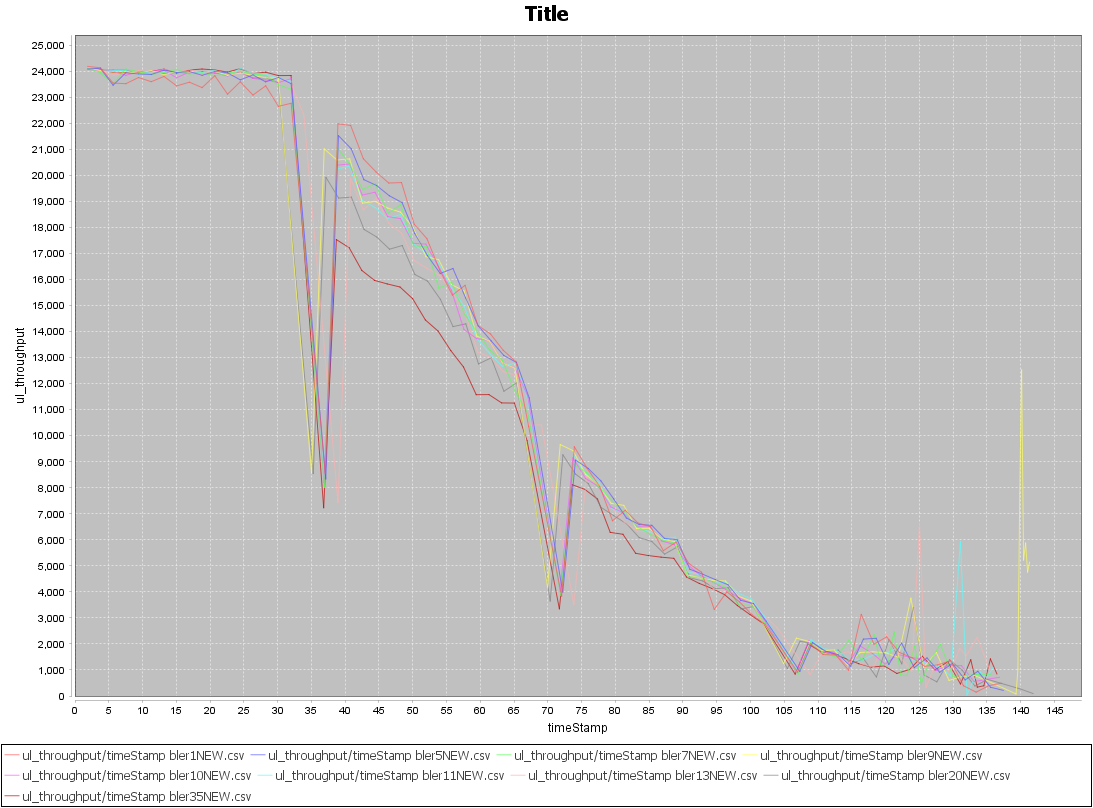
\includegraphics[width=\textwidth]{ulThroughputOverTime}
\centering
\caption{picture of throughput over time}
\end{figure}

The above graph shows how the throughput looks over time. What we can see is that throughput is decreasing over time, as was expected. What is interesting is that after 35 second there is a huge dip in the graph. We thought this was very strange so we studied the csv file (which we plotted the data from) to see if it was something wrong in this file. What we saw was that in all files there was a jump in time, so either the cellphone stopped sending data in this interval or the csv file is generated in wrong way. Otherwise there seems to be a little difference between the throughput curves, the data that has 20\% and 35\% BLER target has lower throughput and that was also our hypothesis but the curves with low BLER target such as 1\% 5\% and 7\% didn't seem to be experience any loss in throughput which is interesting. More detailed graphs are available in appendix chapter X

\newpage
\subsection{Throughput over SINR}

\begin{figure}[h]
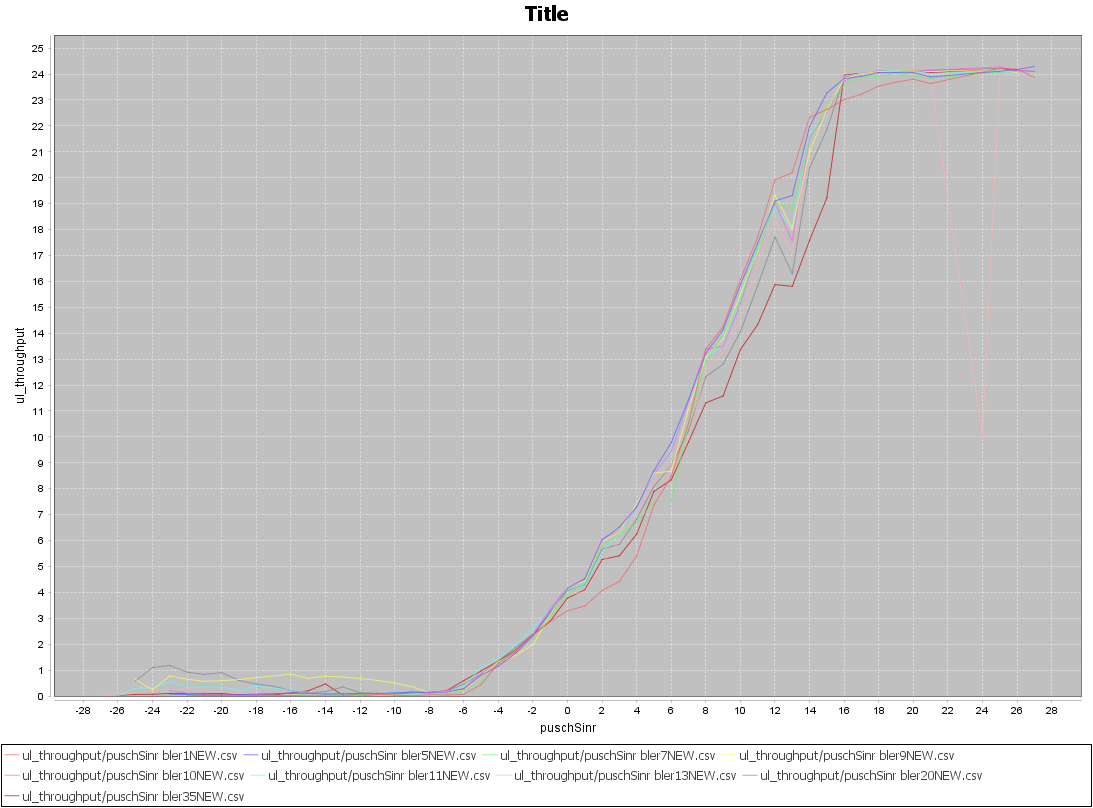
\includegraphics[width=\textwidth]{ulThroughputOverSINR}
\centering
\caption{picture of throughput over SINR}
\end{figure}

The above picture show how the throughput over SINR looks. What we can see is that the throughput is decreasing when the SINR is decreasing. What look strange in this graph is that the throughput over SINR 13 seems to be worse than that of SINR 12. We wondered if we might  have written something wrong when we calculated this graph. How we calculated throughput over another parameter thats not time e.g. SINR, is that we sum up all the TBS's that has the same SINR, multiply each TBS with its corresponding HARQ, ACK = 1 and NACK = 0. and divide it with the number of TBS's you've found for these SINR's. We could check if this was correct by using excel, copy bb-filtered data traffic, filter out irrelevant data to see what the throughput was at SINR 12 and 13. It turned out that the throughput was actually lower at SINR 13 than 12. What we also could see was that the throughput seems to be higher for the simulations with lower bler targets at high SINR and that the throughput is higher at low SINR for the simulations with higher BLER target. For a more detailed picture see appendix chapter X.




\newpage
\subsection{BLER and MCS over time}

\begin{figure}[h]
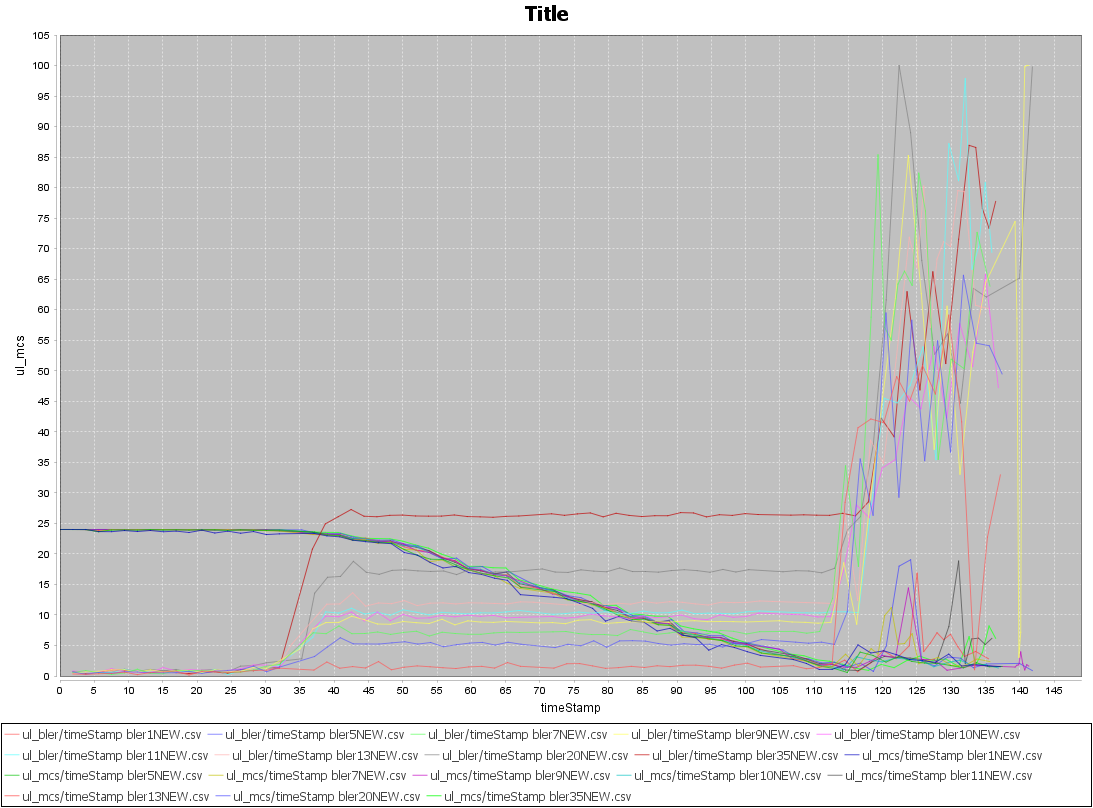
\includegraphics[width=\textwidth]{ulBLER_And_MCS_OverTime}
\centering
\caption{picture of BLER over SINR}
\end{figure}

In the above picture the BLER and MCS over time is showed. What we want to see is if the curves goes as they are intended to do. The link adaptation algorithm states that the mcs will increase if the BLER is under the target, and vice versa. So as stated earlier when the SINR goes down the BLER goes up and then the MCS will drop. So at the time BLER reach its target the mcs should start to drop (since the SINR is decreasing over time). We can see that is does that, which indicates that the graphs are presenting the right data. The BLER Should also hold its assigned target, it seems to do that except for bler target 35\% and 20\%. why this is we don't know. But it seems to be this way for these two simulations, so the graph represent the data in the csv file. When the MCS goes towards zero the BLER goes up which is expected. A more detailed image is available in appendix x.
\newpage
\subsection{BLER over SINR}

\begin{figure}[h]
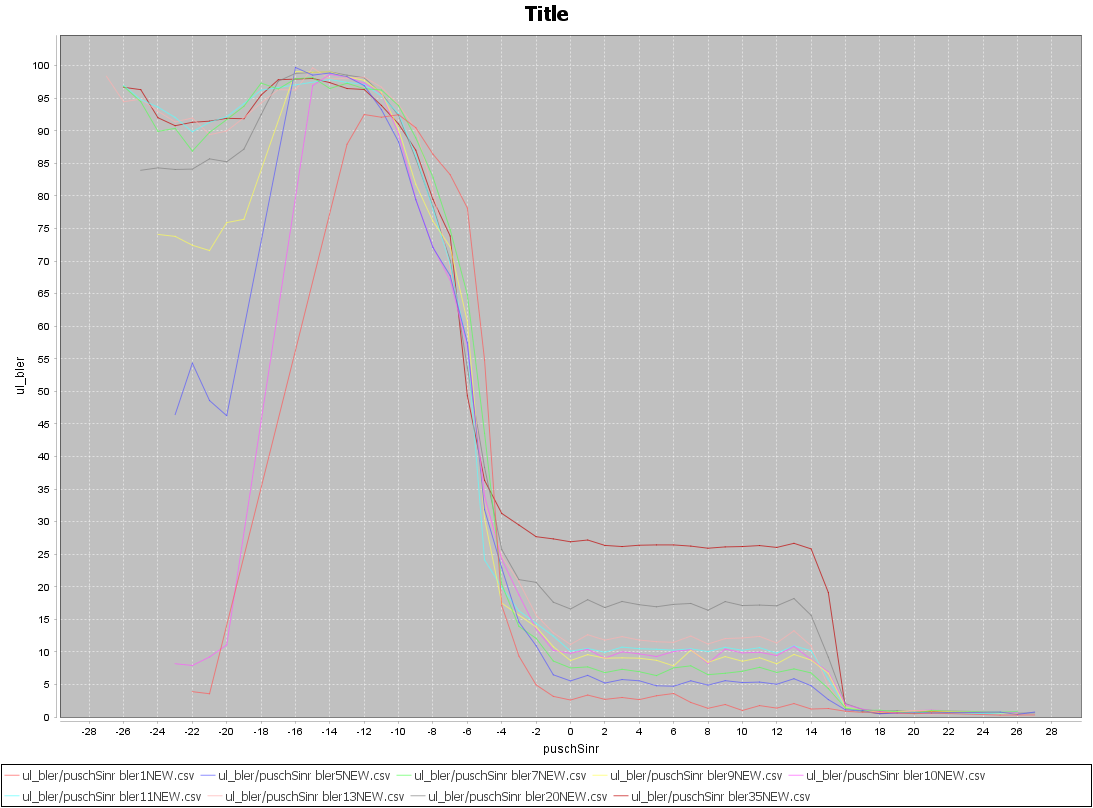
\includegraphics[width=\textwidth]{ulBLEROverSINR}
\centering
\caption{picture of BLER over SINR}
\end{figure}

In the above picture the BLER over SINR is showed. This graph shows that that for the highest SINR the BLER is around zero, then it goes up to each respective BLER target. Then it goes up to 100\%, after that it goes down to towards zero, which seems incorrect, this will be explained later.
\newpage
\subsection{MCS over time}

\begin{figure}[h]
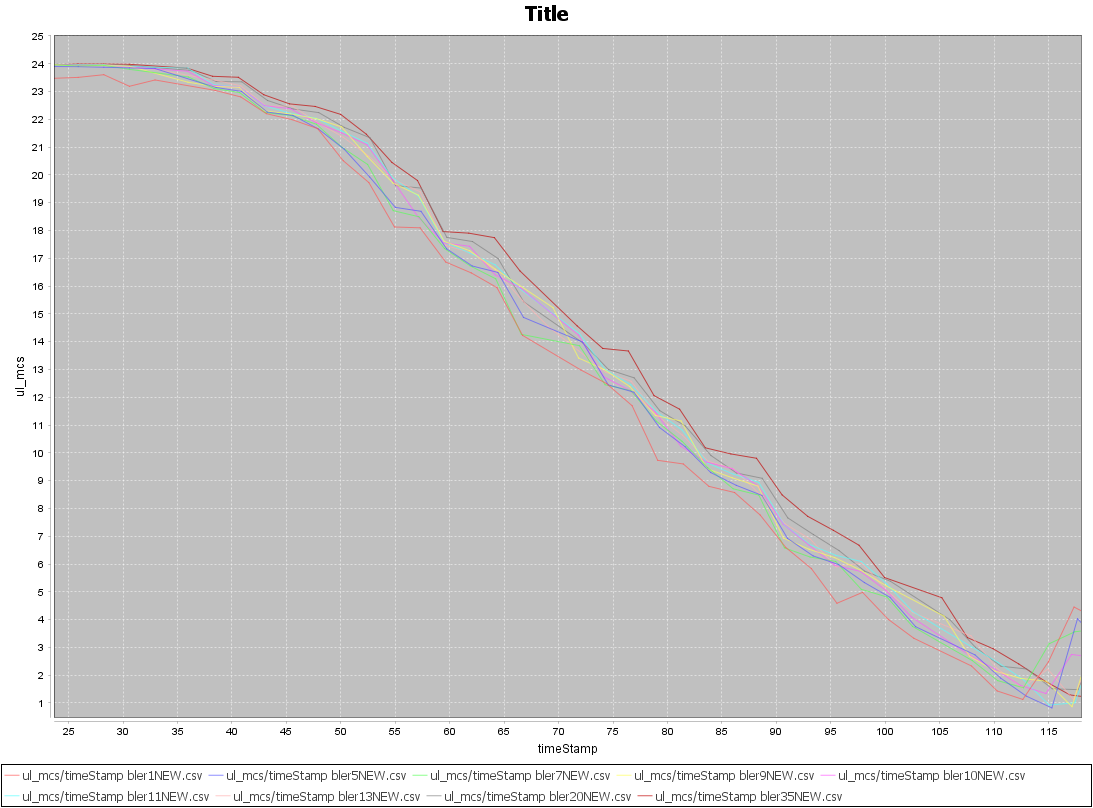
\includegraphics[width=\textwidth]{ulMCSOverTime}
\centering
\caption{picture of MCS over time}
\end{figure}

The above picture should show that the MCS for the higher BLER target simulations are dropping slower than the one of the simulations for the lower BLER target, this was also expected.

\newpage

\subsection{MCS over SINR}

\begin{figure}[h]
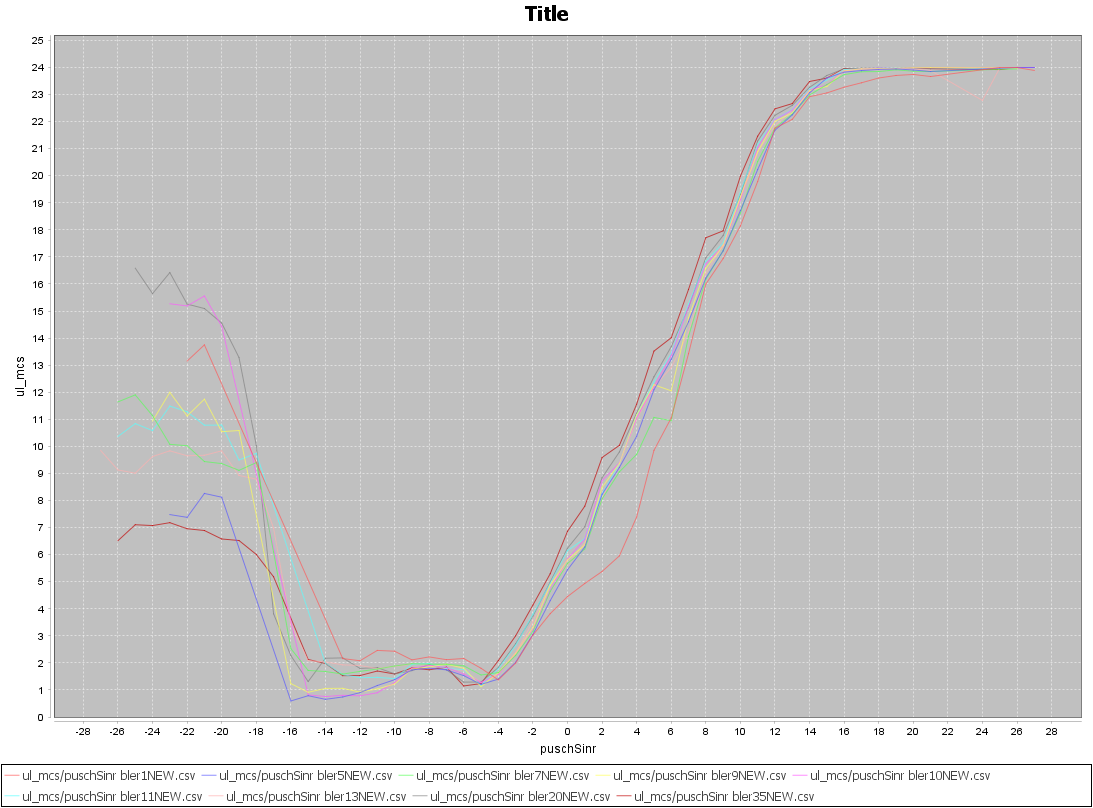
\includegraphics[width=\textwidth]{ulMCSOverSINR}
\centering
\caption{picture of MCS over SINR}
\end{figure}

In this graph MCS over SINR is showed, in the beginning i looks as expected. The MCS values for the simulations with the lower BLER target is dropping faster than the simulations with higher BLER target. At SINRs around -13 dB it the MCS starts to increase. This was not expected and looks wrong. We started investigating the and saw that the SINR in the high region sometimes is dropping from around 20 dB to -20 dB  and then back to 20 dB in the time span of two ms where the MCS is around 24 these, values will contribute when calculating the average of these SINR's. The same reason is why BLER over SINR is going down towards zero at very low SINR's.


\section{Conclusion}
what we did in this analysis was to test whether our tool works as expected and to find erroneous behaviour either inform of incorrect drawing of graphs or in some or in the data. \\

We are able to load different sets of data where the files are quite large, 1.4 gigabytes of data and load 10 of these in the same file

We can also see from the analysis that the different BLER target seems to have an impact on the throughput. The higher BLER target you have the better performance you seem to have at low SINR and the lower BLER target you have the better throughput performance you seem to have at higher SINR's.














\chapter{Future work}
In this area we have experienced that there are not a lot of similar tools. We had many ideas how to further develop this tool to something more useful tool or just to make it better / easier to use. But since we only had a limited time to implement focused on the most relevant parts.\\

The current drawback with the tool is that in able to run it you have to draw a trace, save it to a raw file and then read the file which may overall be quite time consuming. If you want to do a quick analysis or a faster one, you should be able to produce graphs in real time which logtool has support for and from that data produce graphs. This we felt could be very good but we felt that was outside our scope for this thesis. \\

We also feel that it is necessary to adjust the test cases to suit this tool better. Right now the tests that are testing data traffic are based on that the test uses bbfilter. And is something in the line with, check parameter "X" is changing when the SINR is changing. You don't at the moment have test cases that involves analysing all the data traffic only that a parameter is changing under certain circumstances, not the whole data traffic. \\

\section{Unimplemented Work}
There are some things that we wanted to do but we didn't have time to. One is that when you are in advanced view and wants to look at TBS over SINR and and compare it with CQI over SINR, right now you would only see the TBS over SINR graph because the TBS values are in general much larger than CQI values. A solution to this is to do two scales so that both would appear in the window. \\
Another thing is that you could show max and min curves and perhaps other types, right now average curve is the only thing you can watch.

\subsection{Potential new features}

There are a lot of different features that one could add to make the tool more usable.


One other features in advanced view could be when you have chosen what type of data you want to study on one axis, irrelevant data would dissapear to choose from the axis. For example if you want to study uplink throughput at Y-axis you should not be able to set CQI on the X-axis because this is a downlink parameter.

Another feature could be that when hovering over points in the graph would give some more details, one could be from how many values this specific data, the average calculated from.

One could also do more representation of data in the bbfilter columns. Right now we only take care of a few number of non-numbers parameters. One could do more special representations of these if you want to plot over that. Right now the we only take care of NDF and HARQ data. ndf = Y and HARQ = ACK is represented as 1, ndf = N and HARQ = NACK is represented as  0.

There is also relevant to do something about the files that bbfilter translates. They are sometimes erroneous. You could do implement some functionality that corrects it. or at least states the they are erroneous. An example is that the time is not increasing with 1 ms for each line in the csv file which it should to be able to calculate the throughput in a correct way.

When plotting several data in the same window, the graph axis will scale so that the data with the largest value are fitting good. This makes other graph with lower values hard to see unless you zoom. For example if you want to study BLER over time and TBS over time in the same window you would not see the bler graph because it can only contain values between 0 to 100, and TBS between values 0 - 75000. One feature is to scale the graphs such that all graphs are visible in the same window.

We could also add min and max curves. In the beginning we felt it would contain too much data in the basic view to have both max min and average, and like in the downlink cases, there would be 6 graphs in some of the cases, if you then would load data you would have 6 more graphs for each new file you load, so we dropped that idea. This were before we thought of the advanced view. At that time we had forgot it and we felt was too late to implement it when we remembered it again.

There is also the possibility of adding automatic analysis. We began to implement this but we then realized that it might be redundant. We asked our supervisor if this could be good but she said it wasn't necessary. The drawback with adding new functionality is that it might not be used and it might lead to confusion. But it could still be an alternative.  


\chapter{Conclusion} % chapter 7

What we have done in this master thesis was to develop an analysis tool for Ericsson. The purpose was to be able do in-depth analysis on traffic data in the physical layer, which they were not able to do before. What we have developed was a graphical tool that took in two sets of data that comes from a trace file and plot it as a graph. This way one can make more in-depth analysis of physical layer data, especially those of link adaptation. To show that an analysis is possible we did our own analysis on the BLER target which is closely linked to the Link adaptation algorithm [source]. From the result of this tool we can say that we can do ...

\newpage




\chapter*{References}
[1] Teppei Ebihara, Hidekazu Taoka, Nobuhiko Miki, and Mamoru Sawahashi. Performance of Outer-Loop control for AMC based on mutual information in MIMO-ODFM downlink, 2012 \\

[2] Tao Cui, Feng Lu, Anil Goteti, V. Sethuraman, S. P. Rao and P. Subrahmanya. Throughput Optimization in High Speed DownlinkPacket Access (HSDPA), 2009 \\

[3] Erik Dahlman, Stefan Parkvall, John Sk\"{o}ld, Per Bemin. Academic Press 3G Evolution HSPA and LTE for Mobile Broadband 2nd Edition Oct 2008 eBook-DDU. \\

[4] http://www.3gpp.org/technologies/keywords-acronyms/98-lte \\

[5] Ericsson, Ericsson Academy LTE L11 Air Interface, 2011 \\

[6] http://ieeexplore.ieee.org/stamp/stamp.jsp?tp=\&arnumber=5741922 \\ %performance of LA

[7] 3GPP TS 36.300 V12.2.0 , p34\\

%[8] ftp://www.3gpp.org/tsg_ran/WG1_RL1/TSGR1_19/Docs/PDFs/R1-01-0237.pdf

\end{document}

